\documentclass[11pt]{article}
\title{\textbf{Meccano fox frame}}
\author{https://github.com/heptagons/meccano/frames/fox}
\date{}

\usepackage{../../meccano}
\usepackage{tikz}
\usetikzlibrary{calc}

\begin{document}

\maketitle
\begin{abstract}
Meccano fox frame is a group of five meccano\meccanoref strips intended to be a
base to build equilateral polygons. It resembles a fox face with two big pointing ears.
The frame was used to build a regular pentagon\footnote{
\href{https://github.com/heptagons/meccano/tree/main/penta/pentagons.pdf}{Meccano pentagons}	
} and here we explore more polygons.
We conjecture the fox frame permits to build only a single pentagon, infinite hexagons,
but no octagons, decagons nor dodecagons according to a brute-force search.
\end{abstract}

\begin{figure}[htb]
\centering
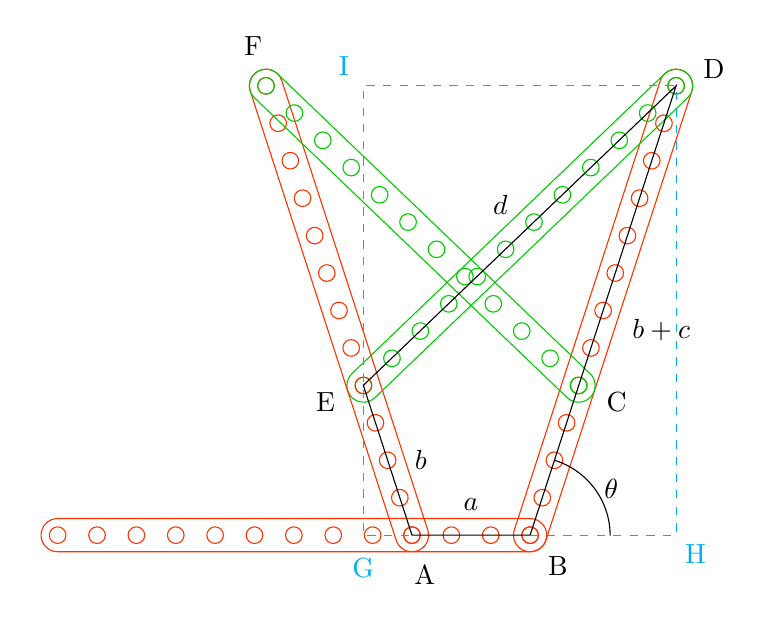
\begin{tikzpicture}

\newcommand{\rod}[4][000000] % [color][n][sep][prop]
{
 \definecolor{main}{HTML}{#1}
 \draw[main] (0,{{2*#4}})
   -- ++({#2*#3},0) arc(+90:-90:{2*#4})
   -- ++({-#2*#3},0) arc(270:90:{2*#4});
 \foreach \x in {0,1,...,#2}
  \draw[main] (\x*#3,0) circle (#4);
}

\def\s {12} \def\f {0.5} \def\p {3pt}
\def\red {FF3300} \def\blue {0000cc} \def\green {00cc00}
\begin{scope}
 \rod[\red]{\s}{\f}{\p} \path (0,0) ++(240:5*\p) node{};
 \begin{scope}[shift={(\s*\f,0)},rotate=72]
  \rod[\red]{\s}{\f}{\p} \path (0,0) ++(240:5*\p) node{B};
  \draw[black] (2*\f,0) arc (2*\f:-72:2*\f) node[midway,above,right]{$\theta$};
  \begin{scope}[shift={(\s*\f,0)},rotate=180-28.2]
   \rod[\green]{11}{\f}{\p}
   \path (11*\f,0) ++(-20:5*\p) node{E};
  \end{scope}
  \begin{scope}[shift={(\s*\f,0)},rotate=72]
   \path (0,0) ++(240:5*\p) node{D};
  \end{scope}
 \end{scope}
 \begin{scope}[shift={(9*\f,0)},rotate=72+36]
  \rod[\red]{\s}{\f}{\p}
  \path (0,0) ++(-180:5*\p) node{A};
  \path (\s*\f,0) ++(0:5*\p) node{F};
  \begin{scope}[shift={(\s*\f,0)},rotate=180+28.2]
   \rod[\green]{11}{\f}{\p}
   \path (11*\f,0) ++(20:5*\p) node{C};
  \end{scope}
 \end{scope}

\end{scope}

\pgfmathsetmacro{\cosA}{cos(72)}
\pgfmathsetmacro{\sinA}{sin(72)}

\def\a{12*\f}
\def\c{4*\f}
\def\ab{9*\f} % a - b
\coordinate (F) at (\ab,0);
\coordinate (B) at (\a,0);
\coordinate (L) at (\a  + \a*\cosA, 0);
\coordinate (C) at (\a  + \a*\cosA, \a*\sinA);
\coordinate (K) at (\ab - \c*\cosA, \a*\sinA);
\coordinate (I) at (\ab - \c*\cosA, \c*\sinA);
\coordinate (J) at (\ab - \c*\cosA, 0);
\draw[black] (F) 
-- (B) node [midway,shift={(0,1.1em)}]{$a$}
-- (C) node [midway,shift={(+2.1em,-.7em)}]{$b+c$}
-- (I) node [midway,shift={(-.7em,1.1em)}]{$d$}
-- (F) node [midway,shift={(1.2em,0)}]{$b$};
\draw[dashed,cyan] (B) 
-- (L) node[shift={(.7em,-.7em)}]{H} 
-- (C)
-- (K) node[shift={(-.7em,.7em)}]{I} 
-- (I)
-- (J) node[shift={(0,-1.2em)}]{G}
-- (F);    
\end{tikzpicture}
\caption{Fox-figure}
\label{fig:fox-face}
\end{figure}

Figure \ref{fig:fox-face} show the so called meccano fox frame.
Has five strips of three types:
\begin{itemize}
\item Single $\overline{AB}$ of length $a$.
\item Pair \{ $\overline{BD}$, $\overline{AF}$ \} of length $b+c$.
\item Pair \{ $\overline{DE}$, $\overline{CF}$ \} of length $d$.
\end{itemize}
In other words we have four different distances:
\begin{itemize}
\item $a$ distance of segment $\overline{AB}$.
\item $b$ distance of segments $\overline{BC}$ and $\overline{AE}$.
\item $c$ distance of segments $\overline{CD}$ and $\overline{EF}$.
\item $d$ distance of segments $\overline{DE}$ and $\overline{CF}$.
\end{itemize}
We are going to test several values of $(a,b,c,d)$ and calculate the angle $\angle{HBD}$.
First we'll calculate a formula and then we'll run a program iterating integer values.

\section{Algebra}
From figure \ref{fig:fox-face} we define $\theta$ = $\angle{HBD}$ and calculate sines and cosines:
\begin{align}
\theta &\equiv \angle{HBD} = \angle{GAE}\\
\overline{BH} &= (b+c)\cos{\theta}\\
\overline{DH} &= (b+c)\sin{\theta}\\
\overline{AG} &= b\cos{\theta}\\
\overline{EG} &= b\sin{\theta}
\end{align}
We calculate $d$ in function of $(a,b,c)$:
\begin{align}
d^2 &= (\overline{DE})^2 \nonumber\\
 &= (\overline{DI})^2 + (\overline{EI})^2 \nonumber\\
 &= (\overline{AG} + \overline{AB} + \overline{BH})^2 + (\overline{DH} - \overline{EG})^2\\
 &= (b\cos{\theta} + a + (b+c)\cos{\theta})^2 + ((b+c)\sin{\theta} - b\sin{\theta})^2\\
 &= (a + (2b+c)\cos{\theta})^2 + (c\sin{\theta})^2)\nonumber\\
 &= a^2 + 2a(2b+c)\cos{\theta} + (2b+c)^2\cos^2{\theta} + c^2\sin^2{\theta}\nonumber\\
 &= a^2 + 2a(2b+c)\cos{\theta} + (4b^2 + 4bc + c^2)\cos^2{\theta} + c^2\sin^2{\theta}\nonumber\\
 &= a^2 + 2a(2b+c)\cos{\theta} + (4b^2 + 4bc)\cos^2{\theta} + c^2\nonumber\\
 &= 4b(b + c)\cos^2{\theta} + 2a(2b+c)\cos{\theta} + a^2 + c^2
\end{align}
We solve for $\cos{\theta}$ with the quadratic formula:
\begin{align}
\cos{\theta} &= \frac{-2a(2b+c) \pm \sqrt{4a^2(2b+c)^2 - 16b(b+c)(a^2 + c^2 - d^2)}}{8b(b+c)} \nonumber\\
 &= \frac{-a(2b+c) \pm \sqrt{a^2c^2 + 4b(b+c)(d^2-c^2)}}{4b(b+c)}
\end{align}

\subsection{Test pentagon known case}
Meccano fox frame appears in the single solution found of the meccano regular pentagon type 1 construction.
In this case we have $a=3$, $b=4$, $c=8$ and $d=11$. Applying these values in the last equation we have:
\begin{align}
\cos{\theta} &= \frac{-48 \pm \sqrt{11520}}{192} \nonumber\\
 &= \frac{-1 \pm \sqrt{5}}{4}
\end{align}
Since $\cos{2\pi/5} = (\sqrt{5} - 1)/4$ the equation for $\cos{\theta}$ passes the pentagon's test.

\subsection{Meccano fox frame possible polygons}

\begin{table}[h]
\centering
\begin{tabular}{|c c c c c|}\hline
 Polygon & $\angle{ABC}$ & $\theta$ & $\cos{\theta}$ & $\{A,B,C,D\}$\rule[-2ex]{0pt}{6ex}\\ \hline\hline
 Pentagon & $72^\circ$ & 
 $\dfrac{2\pi}{5}$ & $\dfrac{\sqrt{5}-1}{4}$ & $\{4,-1,1,5\}$ \rule[-2ex]{0pt}{6ex}\\ \hline
 Hexagon & $120^\circ$ &
 $\dfrac{\pi}{3}$ & $\dfrac{1}{2}$ & $\{2,1,0,0\}$ \rule[-2ex]{0pt}{6ex}\\ \hline
 Octagon & $135^\circ$ &
 $\dfrac{\pi}{4}$ & $\dfrac{\sqrt{2}}{2}$ & $\{2,0,1,2\}$ \rule[-2ex]{0pt}{6ex}\\ \hline
 Decagon & $144^\circ$ &
 $\dfrac{\pi}{5}$ & $\dfrac{\sqrt{5}+1}{4}$ & $\{4,1,1,5\}$ \rule[-2ex]{0pt}{6ex}\\ \hline
 Dodecagon & $150^\circ$
 & $\dfrac{\pi}{6}$ & $\dfrac{\sqrt{3}}{3}$ & $\{3,0,1,3\}$ \rule[-2ex]{0pt}{6ex}\\ \hline
\end{tabular}
\caption{Regular polygons with $\cos{\theta}$ of the form $\frac{B+C\sqrt{D}}{A}$
where $A,D \in \bbb N$ and $B,C \in \bbb Z$.}
\label{tbl:polygons}
\end{table}

From figure \ref{fig:fox-face} we notice angle $\angle{ABC}$ can be used as the internal angle
of a regular polygon.
The internal angle is the supplement of angle $\theta$. Since $\cos{\theta}$ is an algebraic number of the form
$\frac{B+C\sqrt{D}}{A}$ we can construct only a small group of regular polygons.
Table \ref{tbl:polygons} list such polygons excluding triangles and rectangles\footnote{
\href{https://en.wikipedia.org/wiki/Exact_trigonometric_values}{Exact trigonometric values}	
}.

\section{Program}

Next program iterates $a,b,c,d$ to find polygons of different sizes.
We set the maximum size to increase the strips lenghts and we get a callback with the
sizes $a,b,c,d$ and the algebraic cosine value of the form $\frac{B+C\sqrt{D}}{A}$. The algorithm prevents repetitions
by scale. We use the package \texttt{github.com/heptagons/meccano/nest} algebra system.
\begin{lstlisting}
func Fox(max N32, found func(a, b, c, d N32, cos *A32)) {
	factory := NewA32s()
	n1 := N32(1)
	for a := n1; a <= max; a++ {
		for b := n1; b <= max; b++ {
			ab := NatGCD(a, b)
			for c := n1; c <= max; c++ {
				abc := NatGCD(ab, c)
				na := N32(4)*b*(b+c)        // 4b(b+c)
				zb := -Z(a)*(2*Z(b) + Z(c)) // -a(2b+c)
				zc := Z(1)                  // 1
				a2c2 := Z(a*a)*Z(c*c)       // a
				for d := c; d <= max; d++ { // d >= c always
					if g := NatGCD(abc, d); g > 1 {
						continue // skip scale repetitions, eg. [1,2,3,4] = [2,4,6,8]
					}
					if zd := a2c2 + 4*Z(b)*Z(b+c)*(Z(d*d) - Z(c*c)); zd < 0 {
						// skip imaginary numbers invalid fox, like d too short
					} else if cos, err := factory.ANew3(N(na), zb, zc, zd); err != nil {
						// silent overflow
					} else {
						found(a, b, c, d, cos)
					}
				}
			}
		}
	}
}
\end{lstlisting}

\newcommand{\foxface}[6]{ % TODO fix Dimension too large for big cases
 \begin{tikzpicture}
 \def\a{#3};\def\b{#4};\def\c{#5};\def\d{#6};\def\bc{#4+#5}
 \pgfmathsetmacro\max{max(#3,#4+#5)} % max(a,b+c)
 \pgfmathsetmacro\aA{-1.0*#3*(2.0*#4+#5)}
 \pgfmathsetmacro\aB{pow(#3,2)*pow(#5,2) + 4.0*#4*(#4+#5)*(pow(#6,2)-pow(#5,2)}
 \pgfmathsetmacro\aC{\aA + sqrt(\aB))/(4.0*#4*(#4+#5))}
 \pgfmathsetmacro\angleA{acos(\aC)}
 \pgfmathsetmacro\angleB{acos((pow(#5,2) + pow(#6,2) - pow(#3+2.0*#4*\aC,2))/(2.0*#5*#6))}
 \begin{scope}
  \meccanostrip[0000FF]{\a}{#1}{#2} %a
 \end{scope}
 \begin{scope}[shift={(#1*\a,0)},rotate=\angleA]
  \meccanostrip[00FF00]{\max}{#1}{#2} % right a > b+c
  \begin{scope}[shift={(#1*\bc,0)},rotate=180-\angleB]
   \meccanostrip[FF0000]{\d}{#1}{#2}; % right d
  \end{scope}
 \end{scope}
 \begin{scope}[rotate=180-\angleA]
  \meccanostrip[00FF00]{\max}{#1}{#2} % left a > b+c
  \begin{scope}[shift={(#1*\bc,0)},rotate=\angleB-180]
   \meccanostrip[FF0000]{\d}{#1}{#2}; % left d
  \end{scope}
 \end{scope}
 \end{tikzpicture}
}

\subsection{Pentagons}
As mentioned above, this program found only a single pentagon. We use this call:
\begin{lstlisting}
func TestFoxPentagons(t *testing.T) {
	max := N32(100)
	fmt.Printf("max-lenght=%d a,b,c,d pentagons:\n", max)
	i := 0
	Fox(max, func(a, b, c, d N32, cos *A32) {
		if cos.Equals(4, -1, 1, 5) { //  cos 72°
			i++
			fmt.Printf("% 3d %d,%d,%d,%d\n", i, a, b, c, d)
		}
	})
}
\end{lstlisting}
And we get the single result $a=3, b=4, c=8, d=11$:
\begin{lstlisting}
max-lenght=100 a,b,c,d pentagons:
  1 3,4,8,11
\end{lstlisting}

\begin{figure}[h!]
\centering
\scalebox{0.5}{\foxface{1}{5pt}{3}{4}{8}{11} % size,factor,a,b,c,d
}
\caption{Meccano fox frame $a=3,b=4,c=8,d=11$. $\theta=72^\circ$.}
\end{figure}


\subsection{Hexagons}
More interesting costructions are the hexagons, since the algorithm found several.
We run and filter the solutions where $\cos{\theta} = 1/2$. In order to build efficient
hexagons we impose another condition $a > b+c$. This way the hexagons size will be $a$
and the number of strips will be small since diagonals will remain inside each hexagon.

\begin{lstlisting}
func TestFoxHexagons(t *testing.T) {
	max := N32(40)
	fmt.Printf("max-lenght=%d a,b,c,d efficient hexagons:\n", max)
	i := 0
	Fox(max, func(a, b, c, d N32, cos *A32) {
		if cos.Equals(2,1) { //  cos 60°
			// Efficient hexagons are those when a > b+c
			if a >= b+c {
				i++
				fmt.Printf("% 3d %d,%d,%d,%d\n", i, a, b, c, d)
			}
		}
	})
}
\end{lstlisting}

We found 42 different hexagons when the maximum strip is of size $40$ as shown in next table.
Each row last four numbers correspond to the lenghts of the strips segments $a,b,c,d$:
\setlength{\columnsep}{200pt}
\begin{multicols}{2}
\begin{lstlisting}
  1 4,1,3,7
  2 9,1,6,14
  3 11,5,5,19
  4 12,4,5,19
  5 13,2,9,21
  6 13,3,5,19
  7 14,1,9,21
  8 14,2,5,19
  9 15,1,5,19
 10 15,1,14,26
 11 17,3,12,28
 12 18,6,11,31
 13 19,1,12,28
 14 19,5,11,31
 15 20,4,11,31
 16 20,13,7,37
 17 21,3,11,31
 18 21,4,15,35
 19 21,11,10,38
 20 21,12,7,37
 21 22,2,11,31
 22 22,3,15,35
 23 22,11,7,37
 24 23,1,11,31
 25 23,1,21,39
 26 23,2,15,35
 27 23,9,10,38
 28 23,10,7,37
 29 24,1,15,35
 30 24,9,7,37
 31 25,7,10,38
 32 25,8,7,37
 33 26,7,7,37
 34 27,5,10,38
 35 27,6,7,37
 36 28,5,7,37
 37 29,3,10,38
 38 29,4,7,37
 39 30,3,7,37
 40 31,1,10,38
 41 31,2,7,37
 42 32,1,7,37
\end{lstlisting}
\end{multicols}
When we extend the maximum size to $100$ we found $350$ hexagons where the last one
has strips $a=84, b=1, c=11, d=91$.

\subsection{Octagons and dodecagons}

The program found no octagons nor dodecagons by calling these two functions (time ellapsed around 116 seconds each):
\begin{lstlisting}
func TestFoxOctagons(t *testing.T) {
	max := N32(80)
	fmt.Printf("max-lenght=%d a,b,c,d octagons:\n", max)
	i := 0
	Fox(max, func(a, b, c, d N32, cos *A32) {
		if cos.Equals(2,0,1,2) { //  cos 45 degrees sqrt{2}/2
			i++
			fmt.Printf("% 3d %d,%d,%d,%d\n", i, a, b, c, d)
		}
	})
}

func TestFoxDodecagons(t *testing.T) {
	max := N32(80)
	fmt.Printf("max-lenght=%d a,b,c,d dodecagons:\n", max)
	i := 0
	Fox(max, func(a, b, c, d N32, cos *A32) {
		if cos.Equals(3,0,1,3) { //  cos 30 degrees sqrt{3}/3
			i++
			fmt.Printf("% 3d %d,%d,%d,%d\n", i, a, b, c, d)
		}
	})
}
\end{lstlisting}

\section{Conjectures}

According to the program results, we conjecture that including the \textbf{fox frame} exist:
A single pentagon, infinite hexagons, zero octagons, zero decagons and zero dodecagons. 

\section{Fox hexagons examples}

Here we build the first hexagons from the list values. The figures are not presented originally in the paper
Meccano hexagons\footnote{
\href{https://github.com/heptagons/meccano/tree/main/hexa/hexagons.pdf}{Meccano hexagons}	
}. In that paper the so-called irregular diagonals connects hexagon's adjacent sides. 
The difference here is that fox diagonals $d$ connects not adjacent sides but skips one. 
From figure \ref{fig:fox-face} we see the irregular diagonal $d$ connects hexagon's side $\overline{FA}$
with side $\overline{BD}$ skipping side $\overline{AB}$.

\setlength{\columnsep}{10pt}
\begin{multicols}{1}
\begin{figure}[H]
\centering
\scalebox{0.5}{\foxface{1}{5pt}{4}{1}{3}{7} % size,factor,a,b,c,d
}
\caption{Meccano fox(4,1,3,7), $\theta=60^\circ$.}
\label{fig:4-1-3-7}
\end{figure}

\begin{figure}[H]
\centering
\scalebox{0.4}{\foxface{1}{5pt}{9}{1}{6}{14} % size,factor,a,b,c,d
}
\caption{Meccano fox(9,1,6,14), $\theta=60^\circ$.}
\label{fig:9-1-6-14}
\end{figure}
\end{multicols}

Figures \ref{fig:4-1-3-7} and \ref{fig:9-1-6-14} show the two first hexagon fox frames. With 
two copies of each unit we can build a complete hexagon, so we'll have 10 strips. The second copy
is rotated $180^\circ$ and the foxes ears get in touch, imagine that. Also, we can remove a
red diagonal and such hexagon remains rigid.
\\\\
Also we can build the hexagon with 9 pieces with three-fold symmetry.
We start taking only three strips from each unit,
namely a semi-unit including the blue strip, one red and one green as seen in the figures.
Then the semi-unit is cloned two times and rotated each $120^\circ$.
Last figures show these reduced and reinforced constructions.

\newcommand{\foxfacehexagon}[6]{ % three foxfacehex frames
 \begin{tikzpicture}
 \def\a{#3};\def\b{#4};\def\c{#5};\def\d{#6};\def\bc{#4+#5}
 \pgfmathsetmacro\max{max(#3,#4+#5)} % max(a,b+c)
 \def\aC{0.5} % here we prevent dimension error knowing cos=1/2 for hexagons
 \pgfmathsetmacro\angleA{acos(\aC)} 
 \pgfmathsetmacro\angleB{acos((pow(#5,2) + pow(#6,2) - pow(#3+2.0*#4*\aC,2))/(2.0*#5*#6))}
 \begin{scope}
  \meccanostrip[880088]{\a}{#1}{#2} %a
 \end{scope}
 \begin{scope}[shift={(#1*\a,0)},rotate=\angleA]
  \meccanostrip[880088]{\max}{#1}{#2} % right a > b+c
  \begin{scope}[shift={(#1*\bc,0)},rotate=180-\angleB]
   \meccanostrip[880088]{\d}{#1}{#2}; % right d
  \end{scope}
  \begin{scope}[shift={(#1*\max,0)},rotate=60] %second iteration
   \begin{scope}
    \meccanostrip[008800]{\a}{#1}{#2} %a
   \end{scope}
   \begin{scope}[shift={(#1*\a,0)},rotate=\angleA]
    \meccanostrip[008800]{\max}{#1}{#2} % right a > b+c
    \begin{scope}[shift={(#1*\bc,0)},rotate=180-\angleB]
     \meccanostrip[008800]{\d}{#1}{#2}; % right d
    \end{scope} 
   \begin{scope}[shift={(#1*\max,0)},rotate=60] %third
   \begin{scope}
    \meccanostrip[884400]{\a}{#1}{#2} %a
   \end{scope}
   \begin{scope}[shift={(#1*\a,0)},rotate=\angleA]
    \meccanostrip[884400]{\max}{#1}{#2} % right a > b+c
    \begin{scope}[shift={(#1*\bc,0)},rotate=180-\angleB]
     \meccanostrip[884400]{\d}{#1}{#2}; % right d
    \end{scope}
   \end{scope}
    \end{scope}
   \end{scope}
  \end{scope}
 \end{scope}
 \end{tikzpicture}
}

\begin{figure}[h!]
\centering
\scalebox{0.6}{\foxfacehexagon{1}{5pt}{4}{1}{3}{7}
}
\caption{Hexagon side 4 with three fox semi-frames (4,1,3,7).}
\end{figure}

\begin{figure}[h!]
\centering
\scalebox{0.4}{\foxfacehexagon{1}{5pt}{9}{1}{6}{14}
}
\caption{Hexagon side 9 with three fox semi-frames (9,1,6,14).}
\end{figure}

\begin{figure}[h!]
\centering
\scalebox{0.3}{\foxfacehexagon{1}{5pt}{11}{5}{5}{19}
}
\caption{Hexagon side 11 with three fox semi-frames (11,5,5,19).}
\end{figure}

\begin{figure}[h!]
\centering
\scalebox{0.3}{\foxfacehexagon{1}{5pt}{12}{4}{5}{19}
}
\caption{Hexagon side 12 with three fox semi-frames (12,4,5,19).}
\end{figure}

\end{document}

